\chapter{Literature Review}

\textit{``Hunger roared up in him like a hopeless lust.\\ 
He walked the ship as though following a chart. Up. Down. Across. Back. Stem. Port. Stern. Starboard. The churning of the waves. \\
The ropes clanking on the masts. The blind of salt water. The wind ripping at the sails.''\\
\textemdash\ ``Star of the Sea'' by Joseph O'Connor}
\vspace{.2cm}

\section{A Brief Famine Outline}

The Irish lumper potato with its excellent ability to grow in poor and wet soils, was the predominant potato variety in pre-famine Ireland. It was introduced to U.K. around 1806 \citep{tucker2016potato}, and rapidly replacing almost all other varieties in the recipes of the poor. Usually, on account of its intolerance of frost, the farmer sows in March or April, and the first early potatoes will be harvested in June, followed by the second early potatoes in July, and the third not later than October. With a 1.32 \% growth in lower class per year in Ireland from the centennial before 1841, in 1845 about 32\% of the arable land in Ireland was already under potato cultivation \citep{solar2015ireland}.

The first record of late blight on potatoes in Ireland is thought to be Dr Lindley's letter in September 16, 1845, with his concern words, he wrote: ``The potato murrain has unequivocally declared itself in Ireland, where will Ireland be in the event of a universal potato rot''? \citep{kelly1995great}. Things were getting worse in 1846, a government documents collection book recorded that: ``the poor Irish lost their potatoes again'' (1 September, 1846) so that ``Many, full many, must this winter leave their homes, and traverse the country in quest of work'' (15 September, 1846). Government employee pointed out a fact, ``to maintain Ireland's population, her agriculture must be greatly improved'' (31 October, 1846). Next year, due to a change in the Poor Law, ``the poorest peasantry were draught to the shore of America'' (18 January, 1847), but didn't seems to release the effect of famine. Later, in newspaper's leading article, reporter wrote: ``eye-witnesses of scores and hundreds of poor creatures actually dying for want a meal'' (8 March, 1847) and all ``landlord, tenure and peasant were in a miserable situation'' (13 March, 1847). Reflection was raising and people started to realized a serious famine come back since 1741 because ``the food that suffered in both years was the same'' (14 April, 1847). Till November, the exodus of the population was getting worse and caused the ``disorder in Ireland'' (November 13, 1847). Finally, because of sharply decrease population, Ireland faced a situation ``Labour is the first price'' (December 30, 1847) \citep{times1880famineletter}.

Throughout the history of the famine and pre-famine period, the role of the Poor Law cannot be ignored. The Poor Law was introduced in Ireland in July 1838 with the blueprint of the Poor Law in England and Wales, and provided for the establishment of 130 trade unions throughout Ireland, where the poor were to be relieved and regulated by the guardians of the trade unions \citep{o1985new}. However, in January 1847, the government pushed for reform of the Poor Law, which exacerbated the ravages of famine in Ireland \textendash\ particularly in the south and west of Ireland. The most significant consequence of the reforms was the almost complete transfer of responsibility and financial pressure for poverty alleviation to local government finances, which in the context of the famine resulted in the complete collapse of the local poverty alleviation system. It is very difficult to objectively assess the role of poverty law, which on the one hand does provide relief to many poor people \citep{mchugh1986famine}, but on the other hand is also characterized by Foucault's theory of power genealogy like ``micro-power'' and the operation of ``bio-politics'', as the 1847 letter reads:

\begin{itemize}
    \item [] \textit{It is true we have been careful not to put forward a poor-law as a mean to supply, but have claimed for it only a place among the means of distributing supplies \textendash\ of promoting employment, and of enforcing upon poverty the care and protection of the labour. Still, if that surplus of unfilled mouths is to be always in front of us, it must be confessed that very little good, after all, will be accomplished.} \citep{thomas1847poorlaw}
\end{itemize}

After 1847, the rate of depopulation slowed and the most difficult period was over. Some scholars have pointed out that the cause of death of the population during this period was more due to diseases brought about by the famine, including dysentery, diarrhea, tuberculosis, fever, and swelling \citep{mokyr2002people}. The 1851 census showed the population declined by approximately 1.62 million after the famine.

From the census data of 1841 and 1851, we can calculate the change in population of the different provinces after the famine, which showed the result that the west and south suffered far more from famine than the east and north  (Figure 2.1). The five counties with the greatest decreases in population are Donegal, Connaught, in the west, 279,601; Cork, Munster, in the south, 209,822; Galway, Connaught, in the west, 125,026; Tipperary, Munster, in the south, 103,986, and Roscommon, Connaught, in the west, 80,155.\ \textit{The freeman's journal} similarly supports this conclusion in its April 27, 1847 article documenting the damage to parishes including Killedy, Toomavara, Abbey, Lorha and Dorrow, etc \citep{freeman1847parishes}. 

\begin{figure}[htbp]
    \centering
    \caption{County Population 1841 \textendash\ 1851}
    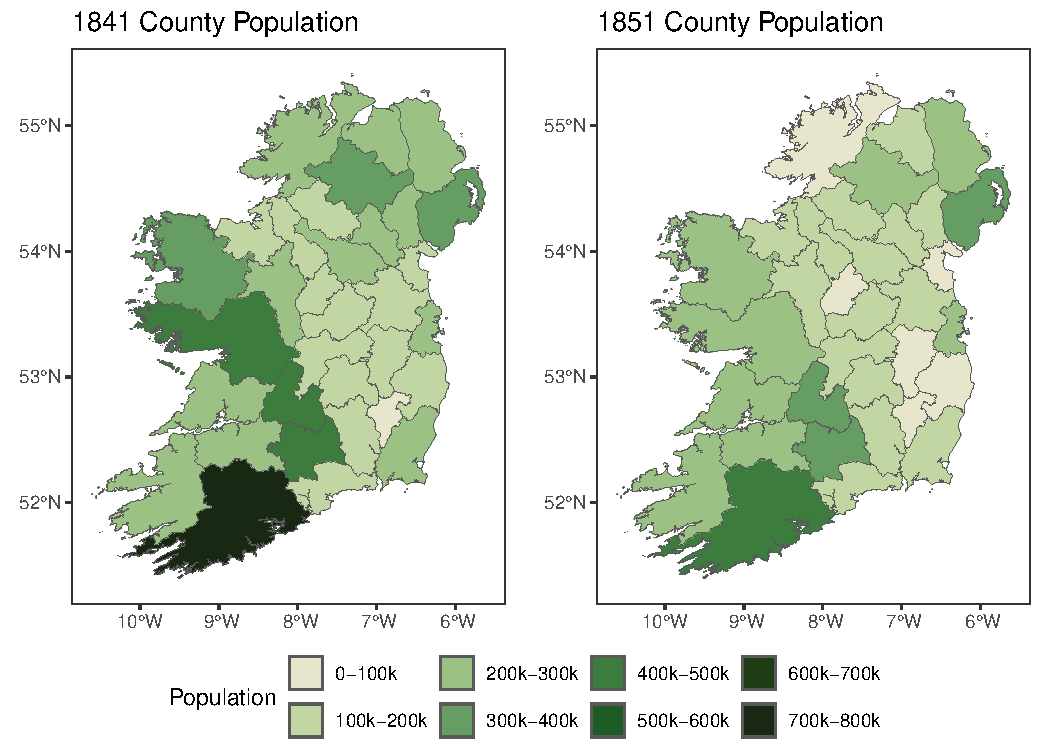
\includegraphics[width=\textwidth]{../03_outputs/map1841_1851.pdf}
\end{figure}

\section{Rebut Food Availability Decline (FAD) Theory}

As Amartya mentioned and argued against in his book \textendash\ ``\textit{the most common approach to famines is to propose explanations in terms of food availability decline (FAD)}'' \citep{sen1982poverty} \textendash\ In the Irish famine, where the FAD theory contains two aspects: (1) the potato late blight; (2) the monocultural structure of the Irish diet. For a long time it was believed that these two were at the root of the famine. In historical fact, while the existence of both is undeniable, their impact is not decisive.

Firstly, potato late blight. During the middle 19th century, late blight and famine have the most intuitive visual connection, so farmers, governments, and scholars have attributed famine to the potato blight. Native Irish farmers have a set of folk myths about this, believing that fairies in the sky were fighting over the potatoes, or that Fear Liath, the fog man, which led to the blight and famine \citep{bartoletti2001black}. Also, references in correspondence with the British government mentioned the relationship between late blight and death in potatoes:

\begin{itemize}
    \item[] \textit{``In 1845, about the month of July or the beginning of August, the potatoes withered and decayed all over the country like what you have seen on
    the watersides with early frost, [\ldots] poor families were badly off and striving to live on bran''.} \citep{mcclureletter1848}
    \item[] \textit{``When they came back home, there was not a potato in what they dug but was infected [\ldots], it is the whole cry among the people''.} \citep{blackwellletter1845}
\end{itemize}

One group of scholars, based on potato production data or biological research, attributes the Famine to late blight, such as Kinealy, who discusses poorhouses, potatoes, and death; \citep{kinealy1990irish}; or Dowley, who focuses on the relationship between climate and blight fungus \citep{dowley1997potato}; also Ristaino, who analysis the DNA structure of the fungus in the famine period \citep{ristaino2006tracking}; as well as scholars working to biologically analyze the uniqueness of the Irish Late Blight strain worldwide and how it led to the famine \citep{goss2014irish}; and the rampant late blight attributed to faulty planting practices \citep{lidwell2020cultivating}.

However, as many scholars opposed to this view have asked, why did Ireland alone suffer such a significantly famine when the late nineteenth-century epidemics swept across the globe \citep{oleksy46irish, mokyr2013ireland, solar2015ireland, kelly2015ireland, gray2006famine}? Scholars have ample biological and historical evidence to prove that late blight did not originate in Ireland, and that it has suffered much less elsewhere than in Ireland \citep{zadoks2008potato}. A Nature article \citep{bourke1964emergence} on the traceability of potato late blight stated that in the 19th century it was first detected in 1843 in port cities on the east coast of the United States, and then spread to the western part of the Americas. In Europe, the first case of late blight was detected in Belgium in June 1845, before spreading to France, the United Kingdom and Ireland (Figure 2.2).

\begin{figure}[htbp]
    \centering
    \caption{Potato Blight Pathway \& Death Rates, 1843 \textendash\ 1845}
    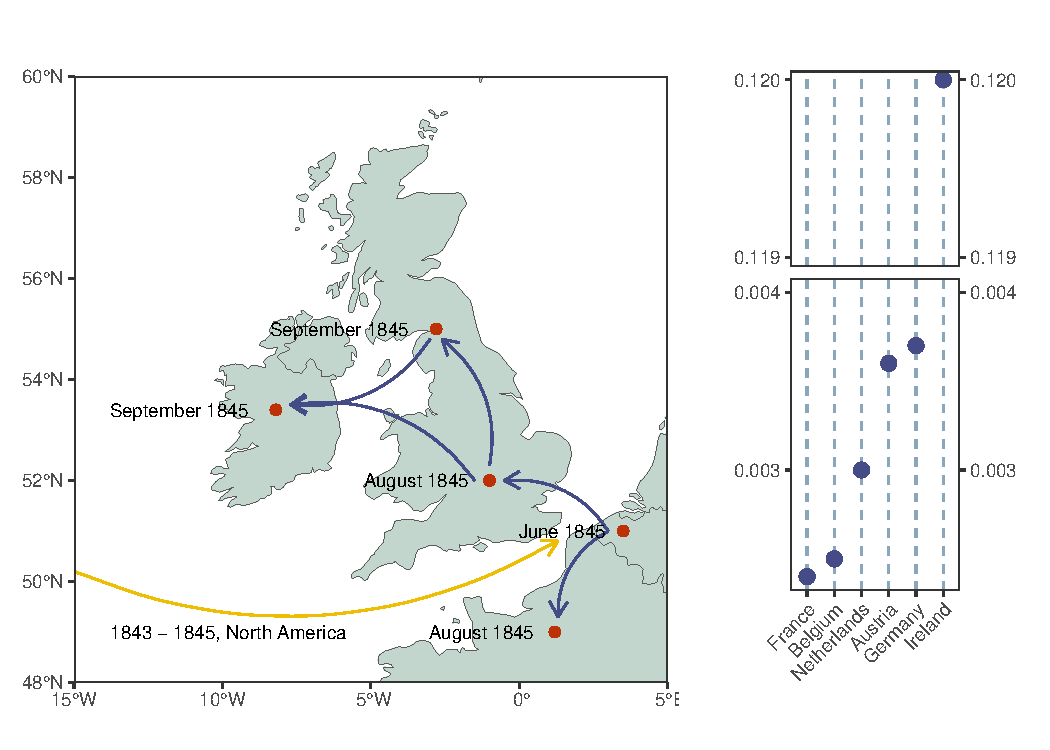
\includegraphics[width=.95\textwidth]{../03_outputs/blight_path_death.pdf}
\end{figure}

There is thus sufficient evidence against the first argument. Since the late potato blight did not strike Ireland first, and since all the other countries afflicted by the blight did not suffer such a great loss of population, the famine directly caused by the late potato blight can not be justified.

Secondly, the monocultural structure of the Irish diet. A strict distinction must be made between the concepts of dietary structure and cropping structure, since the former relates to daily nutritional intake, while the latter relates to the country's agricultural economy at the macro level. When we say “the potato has become almost the only staple food for the poor”, we are actually referring to the former. Ireland in the 19th century was not a country where the potato was almost the only crop, and also there were more than one variety of potato, the lumper. In 1834, when William Cobbett visited the country, he recorded: 

\begin{itemize}
    \item [] \textit{``When men or women are employed, at six-pence a day and their board, to dig Minions or Apple-potatoes, they are not suffered to taste them, but are sent to another field to dig Lumpers to eat''.}\citep{grada1995ireland}
\end{itemize}

For scholars who argue that a monolithic diet led to the famine, they have in fact recognized that Ireland has a diverse cropping structure, it is just that the impoverished poor do not have access to a diverse diet \citep{braa1997great, nally2008coming, de1998famine, kinealy2006great}, which coincides with the entitlement approach that we will address later. And from biological analysis of human proteins \citep{beaumont2014isotopic, beaumont2013victims}, as well as historically documented import and export data \citep{fairlie1965nineteenth}, it is actually clear that the famine victims were given a certain amount of corn as a supplement to potatoes after the famine.

For scholars who argue that a monolithic planting structure led to the famine \citep{turner2002after, bartoletti2001black}, they are ignoring the real historical data, which shows that Ireland was not actually a monoculture potato country at the time. As Popkin rebutted Scott, Irish farmers appear statistically to have been more like rational peasants, and in fact they cut back on potatoes in response to the blight in 1847, shifting to more wheat and oats \citep{o1952food} , which led to a change in the country's overall cropping structure \citep{clarkson2001feast}. Data on Irish cropping structure shows that the country was not as dependent on potatoes as people image, and potato plants proportion at the end of 19th century was more than before famine (Figure 2.3).

\begin{figure}[htbp]
    \centering
    \caption{Grain Agriculture Structure 1820 \textendash\ 1900}
    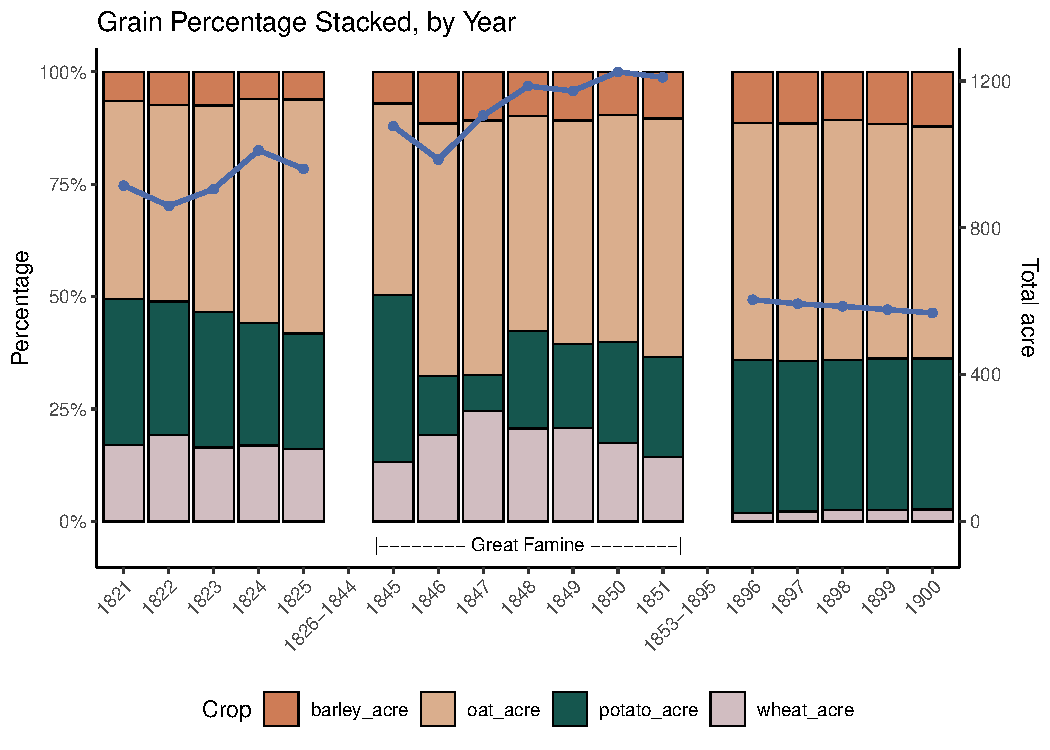
\includegraphics[width=.95\textwidth]{../03_outputs/food_structure.pdf}
\end{figure}

In addition to this, there are a number of explanations that are not directly related to FAD theory but still do not point to the core of the famine, including the problem of poverty in Ireland \citep{gilleard2016other, gray2010irish}, the bad quality of the land \citep{whelan2012clachans} or the cyclical cycle of the famine, but they have corresponding counter arguments respectively, such as studies of Irish immigrants' bank deposits proving that they weren't as poor as they could have been \citep{wegge2017immigrants}, the study of the relationship between land quality and Malthusian metrics \citep{donnelly2002great}, as well as the British government's ability to cope with famine \citep{kelly2015ireland}, etc.

From this we can make the inferences: (1) since potato blight did not originate in Ireland, but was imported via North America, Belgium, and Britain, and since famine losses in other countries were significantly smaller, potato blight was not a central cause of famine; and (2) since the structure of Irish agriculture was not actually entirely monoculture potato, planting structure was not a central cause of famine.

The FAD theory is refuted. Sen's entitlement approach will be discussed next.

\section{Entitlement Approach}

The most widely publicized statement about Amartya Sen's entitlement approach is people are hungry not because they do not have food, but because they are unable to obtain it. There are many other scholars who hold similar views, including Susan George, who discusses emotional indifference, equalization of resources, and unequal systems that led to the famines of the 1980s \citep{george1990ill}; Also Michael Watts interpret famine from a social justice angle \citep{watts2013silent}; and Amrita Rangasami, continue with Sen's entitlement approach, discussed famine in a social welfare, transactions within a community unit like village or family \citep{rangasami1985failure}, etc. Ultimately, Amartya's theory was chosen in this paper, not only because of its widely disseminated, but also for its operationalization level.

Amartya defines the entitlement approach in these four aspects: \textit{(1) Trade-based entitlement, (2) Production-based entitlement, (3) Own-labour entitlement, (4) Inheritance and transfer entitlement} \citep{sen1982poverty}. In fact past studies of the Irish famine have addressed this four aspects, but often lacked a coherent system of entitlement approach.

Firstly, trade-based entitlement. This essentially involves the exchange of a set of ownership pools and market pools, with failure situations consisting of either a deficiency in the ownership pools or a deficiency in the market pools. For food, the former is the sum of the grains within a dietary system, specifically oats, wheat, potatoes and barley in 19th century Ireland, while the latter refers to a market price level. Studies of prices during the famine are common, for example Daniel \citep{daniel2021irish} and Vamplew \citep{vamplew1980grain} focused on oat price, Kennedy and Dowling \citep{kennedy1997prices} researched on potato prices, as well as Clark \citep{clark2004price} in barley price field and Turner's \citep{turner1987towards} paper on a general price index during 19th century. All these papers pointed to price volatility during the famine, which \textendash\ or, using the concepts of entitlement approach, the impairment of trade-based entitlement \textendash\ led to a sharp decline in the market available for Irish, and finally the famine.

Secondly, production-based entitlement. The place of land as an important means of production in the 19th century in the process of granting entitlement to peasants cannot be ignored. Scholars agreed Ireland's 19th century situation as colonial politics \citep{duffy2017colonial, cairns1988writing, nally2008coming} precisely because of the widespread rise of absentee landlords, which created a sharply delineated hierarchy between Ireland and Scotland or England, i.e., peasant \textendash\ attendance landlord \textendash\ absence landlord \citep{braa1997great}. The fact that the relationship between peasants and landowners is obscure and ambiguous probably relates to the wider topic of rural sociology, which, in terms of specific literature, has both an idyllic aspect, such as the peaceful coexistence documented by Brown \citep{brown1953nationalism}, as well as a rhapsodic-like conflict and revolt, such as the land wars of the second half of 19th century.

The uncertainty of the peasant-landlord relationship makes it necessary for this paper to turn its attention to other indicators-namely, taxes and land rents to quantify production-based entitlement. Much of the research on taxation has focused on the tithe, which was enacted from 1823, adjusted in 1838 and finally abolished in 1869. For the first stage (1823 \textendash\ 1838), scholars have focused on the widespread oppression it inflicted on peasants \citep{shaw2015economic, shaw2018composition}, including its also taxed non-Catholic peasants, which led them angry. For the second phase (1838 \textendash\ 1869), although the government transferred the peasants' tithes to the landowners, evidence suggests that the landowners actually passed them back to the peasants \citep{brynn1970irish}, and that the peasants' situation was not substantially improved.


Thirdly, own-labour entitlement. wage and ground rent

Lastly, Inheritance and transfer entitlement. import and export, poor law.


\begin{figure}[htbp]
    \centering
    \caption{Grain Price 1821 \textendash\ 1900}
    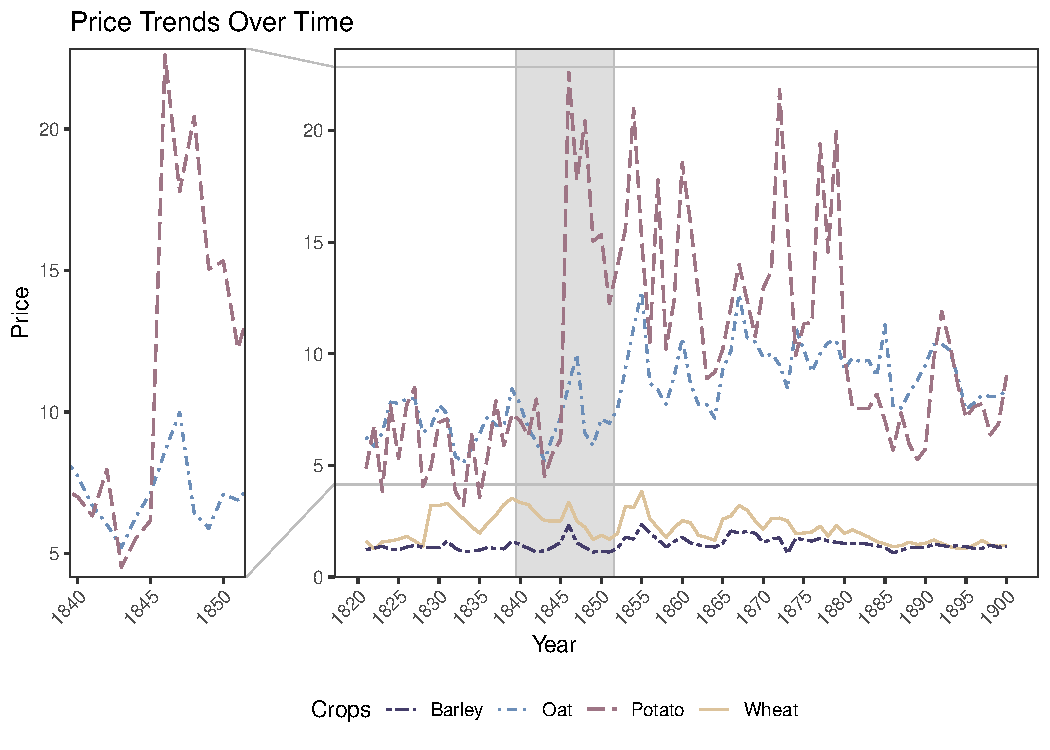
\includegraphics[width=.95\textwidth]{../03_outputs/grain_price.pdf}
\end{figure}




Using Sen's entitlement framework, \citep{fraser2003social}

I n the field of famine studies, scholars as diverse asSusan George (1980), Amartya Sen (1981, 2000),Michael Watts (1983), Amrita Rangasami (1985),and Stephen Devereux (2001) have argued that faminesdo not necessarily begin with crop failures, droughts, orequivalent climatic hazards. On the contrary, their vi-olence is coordinated much earlier when a populationis progressively brought to the point of collapse. Readthis way, a crop failure, or indeed a drought, is simply an“environmental trigger” in a much larger narrative of ag-gregated poverty and mass vulnerability (George 1984;Devereux 2002). Despite the fact that the Great IrishFamine is now a major field of scholarly enquiry, therehas been very little attempt to engage with these criti-cal perspectives—derived primarily from famine expe-riences in the global South—nor has there been any at-tempt to analyze the Great Famine from the perspectiveof colonial governance and population management. \citep{nally2008coming}


I will operationalize entitlement approach into these 4 dimensions according to the book:

(1) trade-based entitlement: price, grain amount, 

(2) production-based entitlement: tax policy

(3) own-labour entitlement: wage, land own amount, poor law

(4) inheritance and transfer entitlement: none, hard to get data






